\section{Simulation of Charpy impact test using \bullet}
\label{sec:bullet-charpy}

In following sections various methods for handling plasticity are described.
As physics engines have not been traditional area of research for plasticity, 
well known Charpy impact test was selected to be used as primary scenario
although it is against first two tips in \bullet Manual.

\begin{itemize}
\item Avoid very small and very larger collision shapes
\item Avoid large mass ratios
\end{itemize}

\subsection{Introduction to constraint processing in \bullet}
Constraint processing in \bullet is based on ODE, \cite{ode}.
Mathematical background and detailed examples are available by \cite{ode.joints}.
Equations \ref{eq:constraintEquation}, \ref{eq:lambdaLow} and
\ref{eq:lambdaHigh} 
are created for each constraint.

\begin{equation} \label{eq:constraintEquation}
J_1 v_1 + \Omega_1 \omega_1 + J_2 v_2 + \Omega_2 \omega_2 = c + C \lambda
\end{equation}

\begin{equation} \label{eq:lambdaLow}
\lambda \geq l
\end{equation}

\begin{equation} \label{eq:lambdaHigh}
\lambda \leq h
\end{equation}

Main parameters  and corresponding fields in \bullet 
 are described in table \ref{tab:constraintParameters}.

\begin {table}[htb!]
\begin{center}
\begin{tabular}{|c| l| l|}
\hline
{\bf Parameter} & {\bf Description} & {\bf btConstraintInfo2 pointer}\\  \hline
$J_1$ & Jacobian & m\_J1linearAxis, m\_J1angularAxis \\ 
$J_2$ & & m\_J2linearAxis, m\_J2angularAxis \\ \hline
$v$ & linear velocity & \\ \hline
$\omega$ & angular velocity & \\ \hline
$c$        &  right side vector   & m\_constraintError \\ \hline
$C$  & constraint force mixing & cfm \\  \hline
$\lambda$ & constraint force &  \\ \hline
$l$ & low limit for constraint force & m\_lowerLimit \\ \hline
$h$ & high limit for constraint force & m\_upperLimit \\ \hline
\end {tabular}
\end{center}
\caption {Constraint parameters} \label{tab:constraintParameters} 
\end {table}

\subsection{Common data}

\subsubsection{Material}

Material is steel. Density is 7800 $kg\over{m^{3}}$. Young’s modulus is 200 GPa. Yield stress is initially 400 MPa but it can be modified.
Coefficient of restitution can be modified and has value of 0 unless otherwise staten.

\subsubsection{Coordinate system}

X axis is horizontal, positive to direction where hammer comes from (left)\\
Y axis is vertical, positive up\\
Z axis is horizontal and Z=0 is symmetry plane

\subsubsection{Specimen}
Specimen dimensions can modified. Basic measures are 10x10x55 mm with 2 mm notch in middle which is taken into account in calculations. Specimen is positioned symmetrically around z=0, bottom at y=0.2 m and backside at x=0. 
Expected energy loss is product of plastic moment of section, hinge angle needed for specimen to go through supports and 
ultimate tensile strength of specimen. For hinge angle of 1.9 radians and ultimate tensile strength of 400 MPa expected energy 
loss is 122 J. Mass is about 40 g and in most cases it is modelled as two 20 g items. In laboratory tests variation for similar 
specimens is roughly about 10 %; see e.g. http://www.npl.co.uk/upload/pdf/cop06.pdf
Specimen can be subdivided to multiple parts.

\subsubsection{Support anvils}
Support anvils initially have 40 mm open space between them. Their width is 40 mm. 
If specimen bends about 1.9 radians (108 degrees) it will go between anvils. Space between anvils can be changed.

\subsubsection{Hammer}
Hammer is 0.5 m wide and 0.25 m high, thickness is 0.02 m. Mass is 19.5 kg. Hammer and hinge are positioned so that 
impact is horizontal  (global x-direction). Hammer arm is 40x40x500 mm. Hammer thickness can be changed.
Setting it to zero causes hammer not to get added to model. Hammer has modifiable draft. Default value is 0.04 m. 
Arm and draft are not taken into account for mass and inertia calculation.

\subsubsection{Energy calculation}

Energy for whole system is calculated so that potential energy and kinetic energy are calculated in updateEnergy. 
When hammer is resting in low position, energy is 64 J. 

\subsubsection{Breaking of constraints between objects}
For standard \bullet constraints breakingImpulseThreshold (BITh) can be defined. If impulse is larger than set limit constraint is activated. 
This allows object breaking to be simulated with very cheap calculation. 
This method is too simplified for ductile material and developing more precise methods in main objective of this work.  

\subsubsection{Timestep}

Usually bullet simulations are done using fixed time step of 1/60 s i.e. 16.67 ms. 
For this case 17 ms is too large timestep even to keep system stable. For impact time much smaller timestep is needed. 
Real time simulation was tried as option but was removed from code as it did not provide good results.  
Default time step was selected to be 5 ms outside impact time and 0.1 ms during impact. 
Automatic time stepping routine changes timestep so that at angles higher than 0.2 5 ms time step is
used and adjusts it linearly to selected time step between angles of 0.2 and 0.05. If specimen is no
longer at anvil larger timestep is also used.

\subsection{Single rigid body}
This is basic reference case without plasticity. Specimen should stop hammer.

\subsection{Constraint with zero limits}
In this case btGeneric6DofConstraint is used with high and low limits set to zero. 
Constraint is made breakable by setting breakingImpulseThreshold.
This is common technique to provide breakable objects in games and provides visually accetable results for brittle materials.

\subsection{SpringConstraint}
This shows how btGeneric6DofSpringConstraints act in case like this. 
Specimen can absorb very little elastic energy so rotational spring constants are calculated using plastic state i.e.
$W=bh^2/4$ where h=b-0.002m and yield stress is used instead of Young’s modulus for rotational springs.

\subsection{Spring2Constraint}
This basically same as SpringConstraint but uses newer btGeneric6DofSpring2Constraint which has recently appeared in
\bullet. 
Automatic stiffness limitation helps to avoid instability but may make constraint too soft.

\subsection{Hinge constraint with motors}
In this case btHingeConstraint is used.
Angular motor is enabled with target velocity of 0 and maximum motor impulse is set to
be plastic moment multiplied by timestep so that motor resists any rotation.

\subsection{PlasticHingeConstraint}
In this case new btPlasticHingeConstraint is used.
It is modification of btHingeConstraint and was is developed during this work.
PlasticHingeConstraint has additional fields for plasticMoment and previousHingeAngle and 
getAbsorbedEnergy method which returns product of plasticMoment and hingeAngle change.

\subsubsection{MaxPlasticRotation}
MaxPlasticRotation is new term which was introduced to allow efficient way to express ultimate strain in bending.
Implemented constraint has additional fields for maxPlasticRotation and currentPlasticRotation. 
After each step in which rotation angle changes, absolute value of 
angle change is accumulated to currentPlasticRotation. As currentPlasticRotation 
reaches maxPlasticRotation constraint is inactivated and specimen breaks. 
For ductile behaviour maxPlasticRotation could be set to e.g. 3-6 (radians) and for brittle
 behaviour to e.g.0.01-0.1 radians. MaxPlasticRotation is basically rotational stretch under bending moment.
 Basic sample can be tried using paperclip. It can typically handle two bend overs before breaking. 
Sewing machine needle or tooth pick which has same diameter is much harder to bend and it 
often breaks before plastic deformation takes place. 

\subsubsection{Limiting maximum moment in constraint}
btPlasticHingeConstraint::getInfo2InternalUsingFrameOffset is modified so that in case of lostop=histop, 
plasticMoment*timeStep is used as upper and lower limit instead of SIMD\_INFINITY. 

\subsection{ElasticPlasticConstraint}
In this case new bt6DofElasticPlasticConstraint is used.
It is based on SpringConstraint with some modifications

\begin{itemize}
\item internalUpdateSprings is modified so that nonlinear relation between displacements and forces can be defined. 
 If force is smaller than maximum force or moment for given degree of freedom,
  elastic behavior is handled in similar way as spring works. 
  If force is larger, maximum force is used. 
\item constraint breaks if active forces are high enough and plastic reserve has been used
\item frequency ratio of lowest mode and integration is used to limit spring functionality to avoid stability issues. 
 Ratio defines how many steps are needed for one period. 
 If number of integration steps is too low, spring is modified to ignore elastic part.
\end{itemize}

\subsection{ElasticPlastic2Constraint}
This is basically same as elasticPlasticConstraint but uses new bt6DofElasticPlastic2Constraint 
which is based on btGeneric6DofSpring2Constraint.
Get\_limit\_motor\_info2, setAngularLimits and setLinearLimits which are called by getInfo2 are modified. 
SIMD\_INFINITY values are replaced by maximum force values which are transformed to
corresponding impulsed by multiplying forces by integration interval.
btGeneric6DofSpring2Constraint has option limitIfNeeded for stiffness and damping to avoid issues. 
Spring is softened so that 4 steps are used for one step. This is not realistic for typical steel structures. 
In bt6DofElasticPlastic2Constraint plasticity code is activated if frequency is too high for stable solution.
If plasticity is activated due to large spring force or due to high frequency forces constraint error is 
calculated in similar way as for case where upper limit equals lower limit, (m\_currentLimit==3).

\section{Charpy impact test results using \bullet}
\label{sec:bullet-charpy-results}

\subsection{Results for single rigid body}

Timestep of 0.1 ms provides expeced results and specimen bounces hammer back as seen in figure \ref{fig:f1-ok-results}.

\begin{figure}[htb!]
\centering
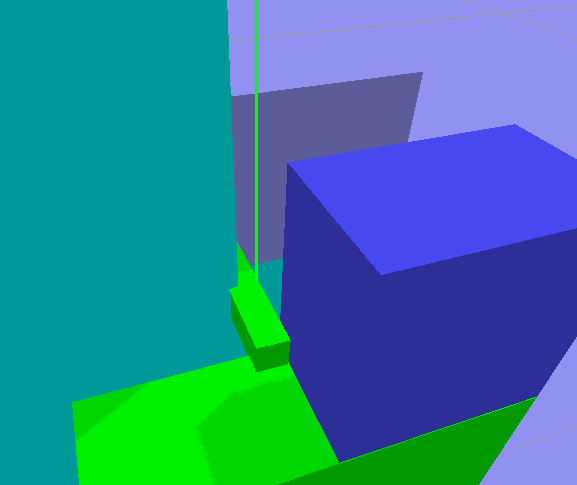
\includegraphics[height=3cm]{figs/f1-18-01-1}
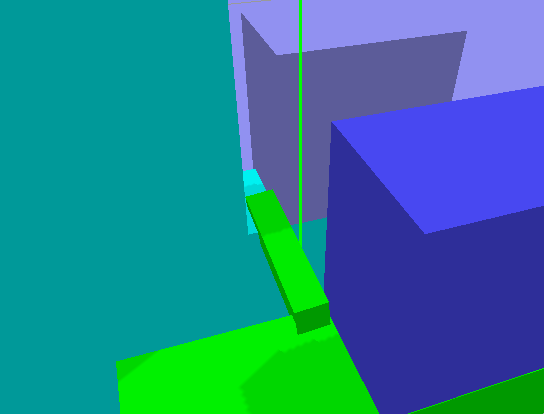
\includegraphics[height=3cm]{figs/f1-18-01-2}
\caption{Specimen bounces hammer back with timestep of 0.1 ms}
\label{fig:f1-ok-results}
\end{figure}

Larger timesteps produce various kinds of unrealistic results seen in figure \ref{fig:f1-nok-results}.
In these cases timestep is 17 ms. Specimen penetrates hammer and anvils.
Without draft specimen stays on anvil.

\begin{figure}[htb!]
\centering
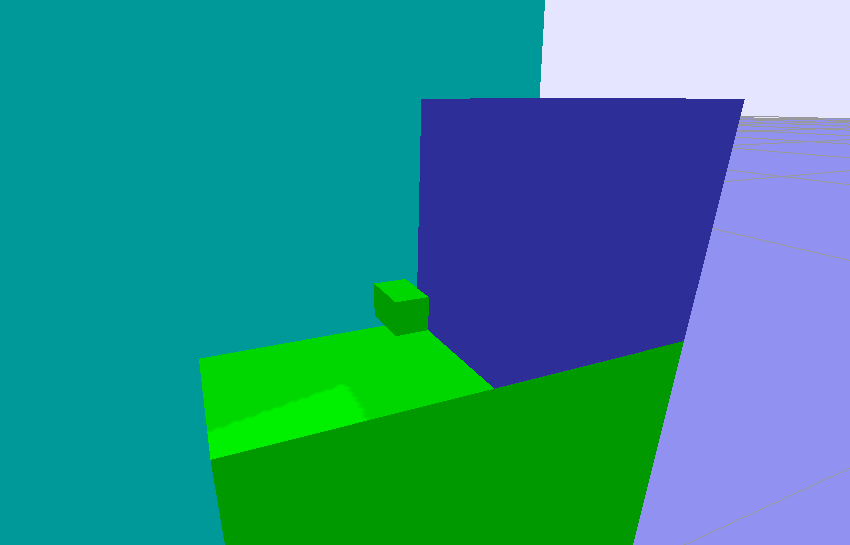
\includegraphics[height=3cm]{figs/f1-18-17-1}
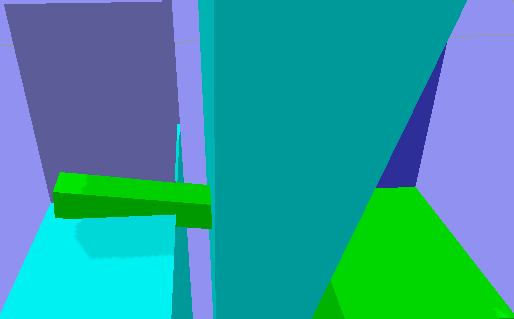
\includegraphics[height=3cm]{figs/f1-18-17-2}
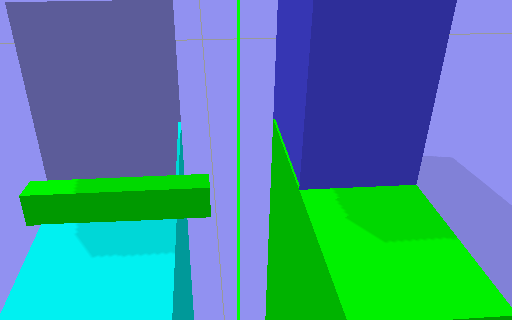
\includegraphics[height=3cm]{figs/f1-18-17-3}
\caption{Results with timestep of 17 ms}
\label{fig:f1-nok-results}
\end{figure}

\subsection{Results for constraint with zero limits}
This technique provides effective and stable way to simulate breaking of brittle material 
but does not provide realistic results for ductile material as can be seen in figure \ref{fig:f3-results}.
Required energy to break constraint can be controlled using
breakingImpulseThreshold. 

\begin{figure}[htb!]
\centering
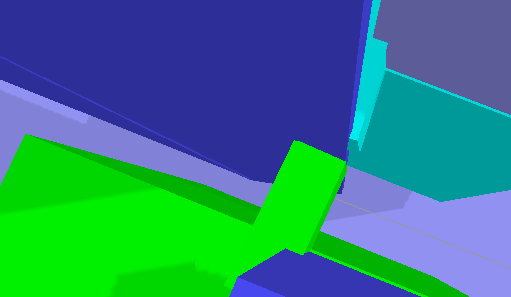
\includegraphics[height=2.5cm]{figs/f3-18-01-1}

\includegraphics[height=2.5cm]{figs/f3-18-01-2}
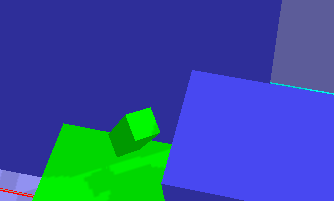
\includegraphics[height=2.5cm]{figs/f3-18-01-3}
\caption{Specimen breaks in brittle way}
\label{fig:f3-results}
\end{figure}


\subsection{Results for springConstraint}
Energy loss is in right scale but visual feedback is not realistic as specimen gets back to initial shape.
Unstable simulation can be seen by setting yield stress to e.g. 800 MPa.

\subsection{Results for spring2Constraint}
Results are quite similar as for springConstraint but automatic parameter tuning helps in avoiding unstable simulations.

\subsection{Results for hinge constraint with motors}
Results are very good although sensitive to parameters changes. Energy loss is in right scale. 
Specimen bends and keeps deformed shape.

\subsection{Results for plasticHingeConstraint}
Results are quite similar as for hinge constraint with motors. 
Breaking point can be configured based on rotation angle which makes material behaviour more realistic.

\subsection{Results for elasticPlasticConstraint}
Results are quite similar as for plasticHingeConstraint as this case is dominated by plastic bending.
Additional logic helps to avoid stablity issues.

\subsection{Results for elasticPlastic2Constraint}
Results are quite similar as for elasticPlasticConstraint and this constraint seems to best candidate for further development.
Table \ref{tab:ep2ts} shows energy loss for few timesteps as example to demonstrate sensitivity of solution.

\begin {table}[htb!]
\begin{center}
\begin{tabular}{| c| c|}
\hline
{\bf Timestep[ms]} & {\bf Energy loss [J]}\\  \hline
 0.100001 &  120 \\ \hline
 0.1 &  110 \\ \hline
 0.09999 &  140 \\ \hline
 0.08 &  170 \\ \hline
 0.05 &  215 \\ \hline
\end {tabular}
\end{center}
\caption {Energy loss for few timesteps} \label{tab:ep2ts} 
\end {table}


\cleardoublepage
